\pdfoutput=1

\documentclass{l4proj}

%
% put any packages here
%
\usepackage{float}
\usepackage{enumitem}
\usepackage{longtable}
\usepackage{listings}
\usepackage{hyperref}
\usepackage{subfiles}
\usepackage{color}
\usepackage{graphicx}
\usepackage{epsfig}
\usepackage{epstopdf}


\newcommand{\nc}[1]{\textcolor{magenta}{(\textbf{NC:} #1)}}
\newcommand{\gac}[1]{\textcolor{cyan}{(\textbf{GAC:} #1)}}
\newcommand{\pwt}[1]{\textcolor{blue}{(\textbf{PWT:} #1)}}

\graphicspath{{images}{../images/}}

\begin{document}
\title{On The Scalability of ROS}
\author{Isaac Jordan}
\date{\today}
\maketitle

\begin{abstract}
Robots, distributed systems, and middleware.
\end{abstract}

\educationalconsent
%
%NOTE: if you include the educationalconsent (above) and your project is graded an A then
%      it may be entered in the CS Hall of Fame
%
\tableofcontents
%==============================================================================

\pagebreak
\pagenumbering{arabic}

\subfile{sections/introduction}

%\vspace{-7mm}
%\begin{figure}
%\centering
%\includegraphics[height=9.2cm,width=13.2cm]{uroboros.pdf}
%\vspace{-30mm}
%\caption{An alternative hierarchy of the algorithms.}
%\label{uroborus}
%\end{figure}

\chapter{Background}
\label{background-chapter}

\subfile{sections/background-part1}

\subfile{sections/background-part2-middleware-overview}

\subfile{sections/background-part3-middleware-discussion}

\subfile{sections/background-part4}

\chapter{Communication Scalability}
\label{communication-chapter}

The communication experiments look in to the scalability of communication in ROS. How well does it handle having to send high frequency work-loads of varying sizes.

\section{Scoping Experiments}

Scoping experiments were quick experiments using dummy data. Designed to identify useful areas to explore in more detail in realistic experiments later.

\subfile{sections/experiment1}

\subfile{sections/experiment2}

\subfile{sections/experiment3}

\subfile{sections/experiment4}

\section{Realistic Data Experiments}

Previous experiments were presented as scoping experiments. These were designed to systematically understand which variables were of concern when running tests on ROS's communication performance. However, it was not certain that these prior conclusions would translate well to using ROS in a realistic scenario. Throughout the scoping experiments, the same message of `hello world' was used as dummy data.

In order to verify the conclusions were correct, samples of realistic data was explored. Two likely data types were settled on, `sensor data' and `video data'.

Sensor data is the type of data likely the come from a physical sensor on the robot. This data is characterised by small message sizes, such as 4KB.

Video data used was a 30Hz (30 frames-per-second) RGB video stream, with a resolution of 640 x 480 pixels. This message stream was measured to use 9.25MB/s of bandwidth, implying a message size of 308KB.

Both data sets were acquired from the MIT Stata Center dataset \cite{mit-stata-center-dataset}. This dataset contains both sensor feeds (such as from a laser sensor), and video feeds (from a Kinect RGB + depth camera). These data sets are very large (20 - 50GB) which would require modification to the test system (Raspberry Pi 3’s). Thus these datasets have been filtered down to 60 seconds of recording, resulting in 1791 camera images, and 1194 LaserScan readings.

\subfile{sections/experiment5}

\subfile{sections/experiment6}

\chapter{Host Scalability}
\label{host-scalability-chapter}

These scalability experiments look in to how well ROS scales when introduced to more nodes, or more hosts, or both.

\subfile{sections/experiment7}

\subfile{sections/experiment8}



\subfile{sections/conclusion}





%%%%%%%%%%%%%%%%
%              %
%  APPENDICES  %
%              %
%%%%%%%%%%%%%%%%
\begin{appendices}

\chapter{Experiment 2 Other Graphs}
\label{exp2-appendix-results}

\begin{figure}
\centering
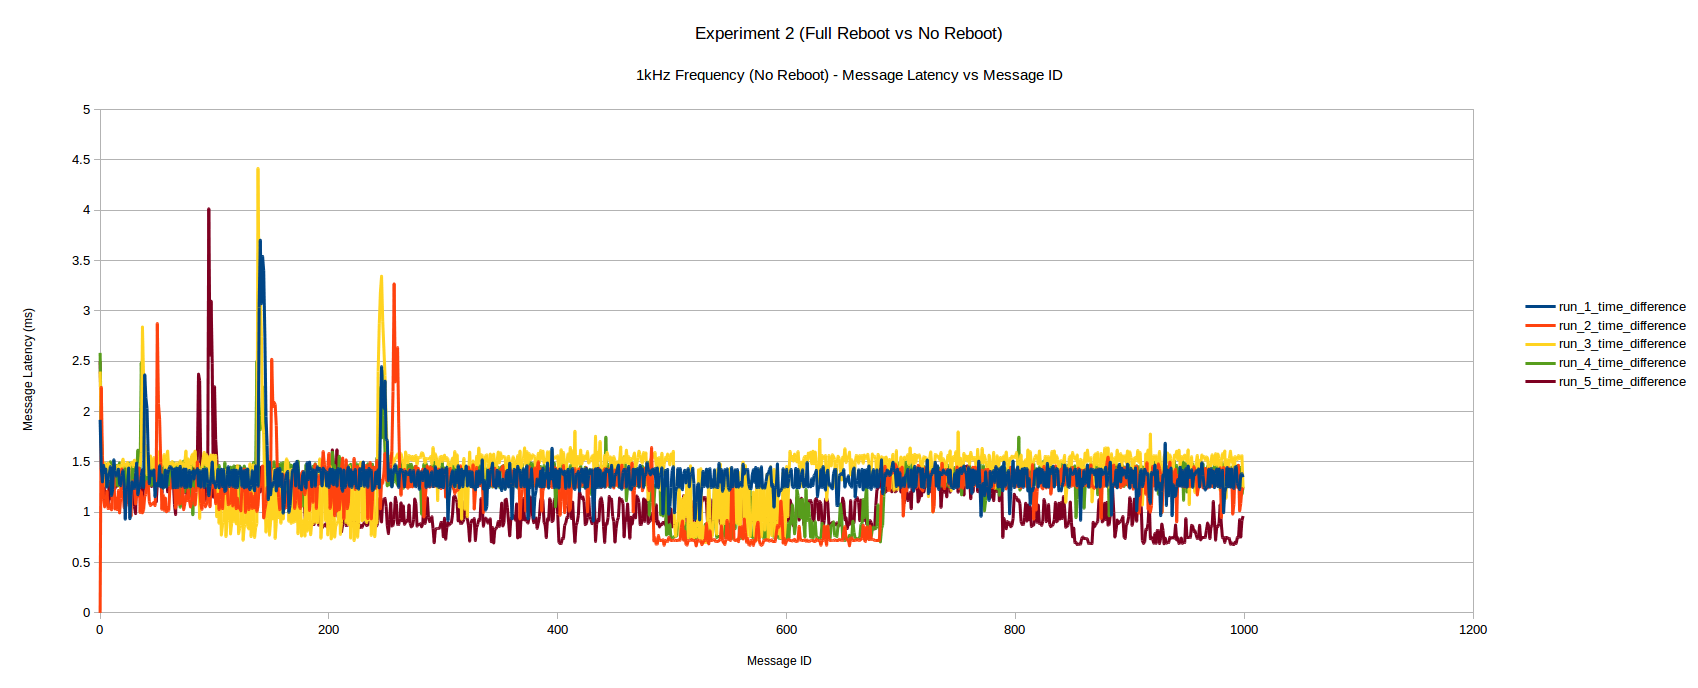
\includegraphics[width=\textwidth]{images/no-reboot-1khz.png}
\caption{Experiment 2 - No Reboot 1KHz Message Frequency}
\label{exp2-noreboot-1khz}
\end{figure}
Other graphs commented out for now.
\iffalse
\begin{figure}
\centering
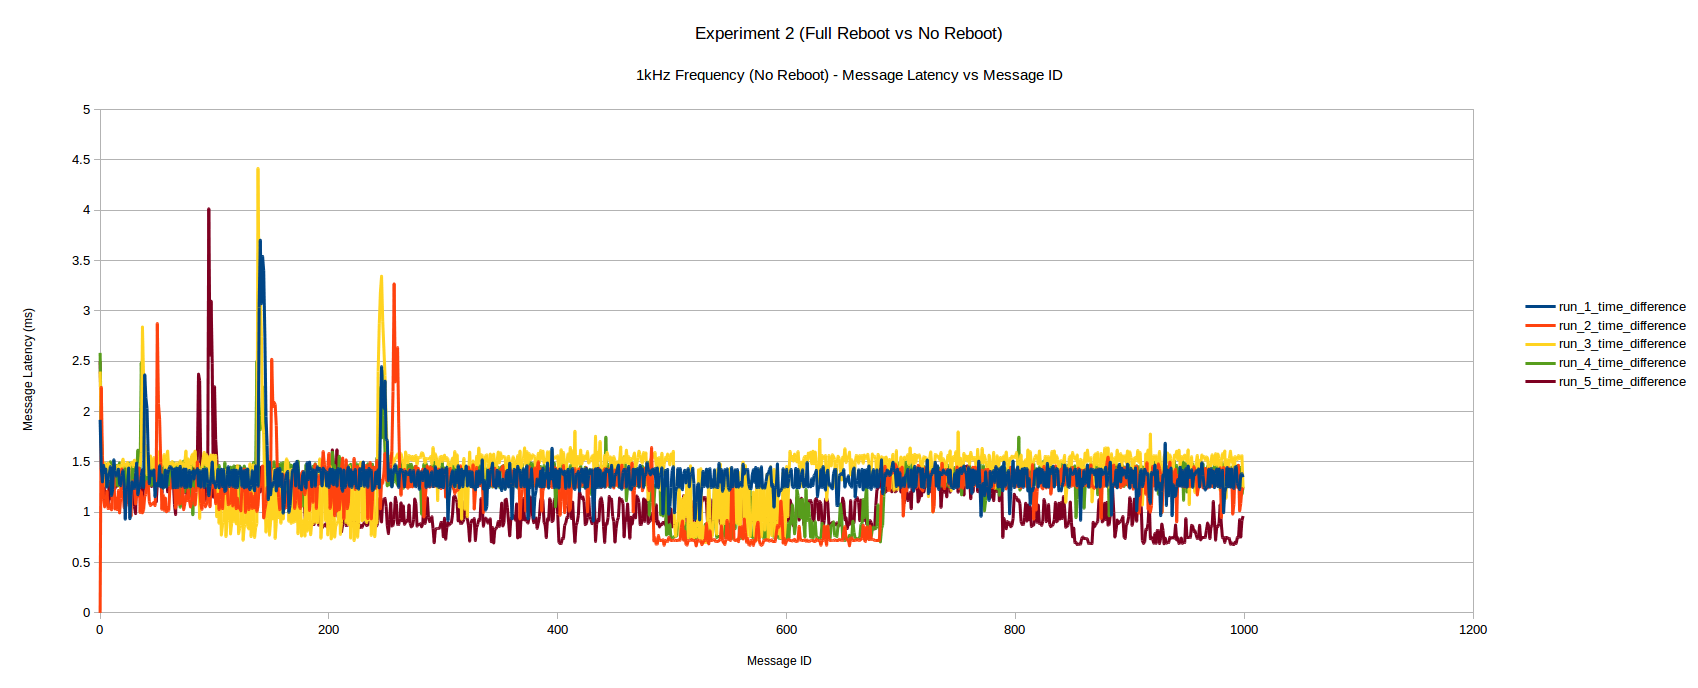
\includegraphics[width=\textwidth]{images/no-reboot-1khz.png}
\caption{Experiment 2 - No Reboot 1KHz Message Frequency}
\label{exp2-fullreboot-1khz}
\end{figure}

\begin{figure}
\centering
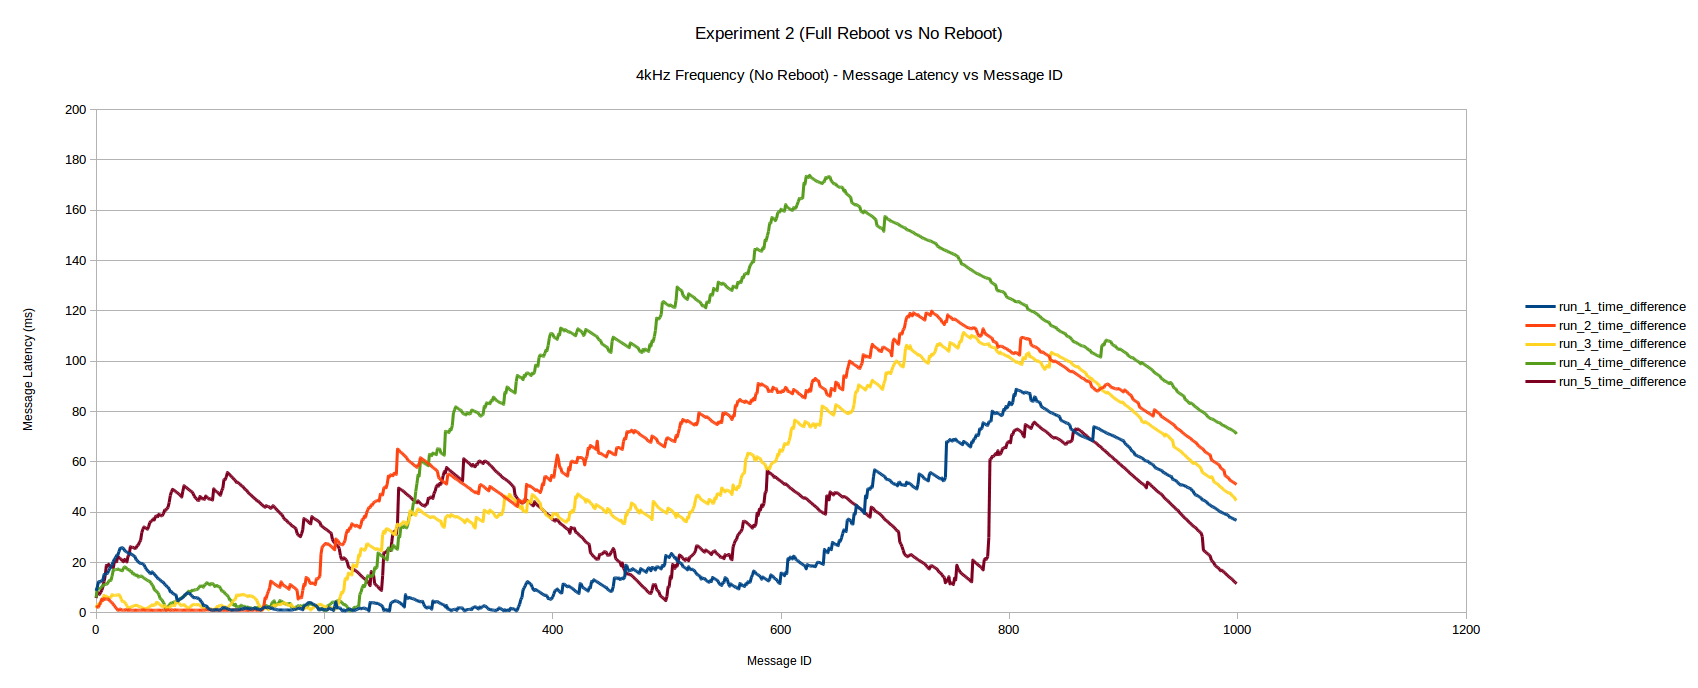
\includegraphics[width=\textwidth]{images/no-reboot-4khz.png}
\caption{Experiment 2 - No Reboot 4KHz Message Frequency}
\label{exp2-noreboot-4khz}
\end{figure}

\begin{figure}
\centering
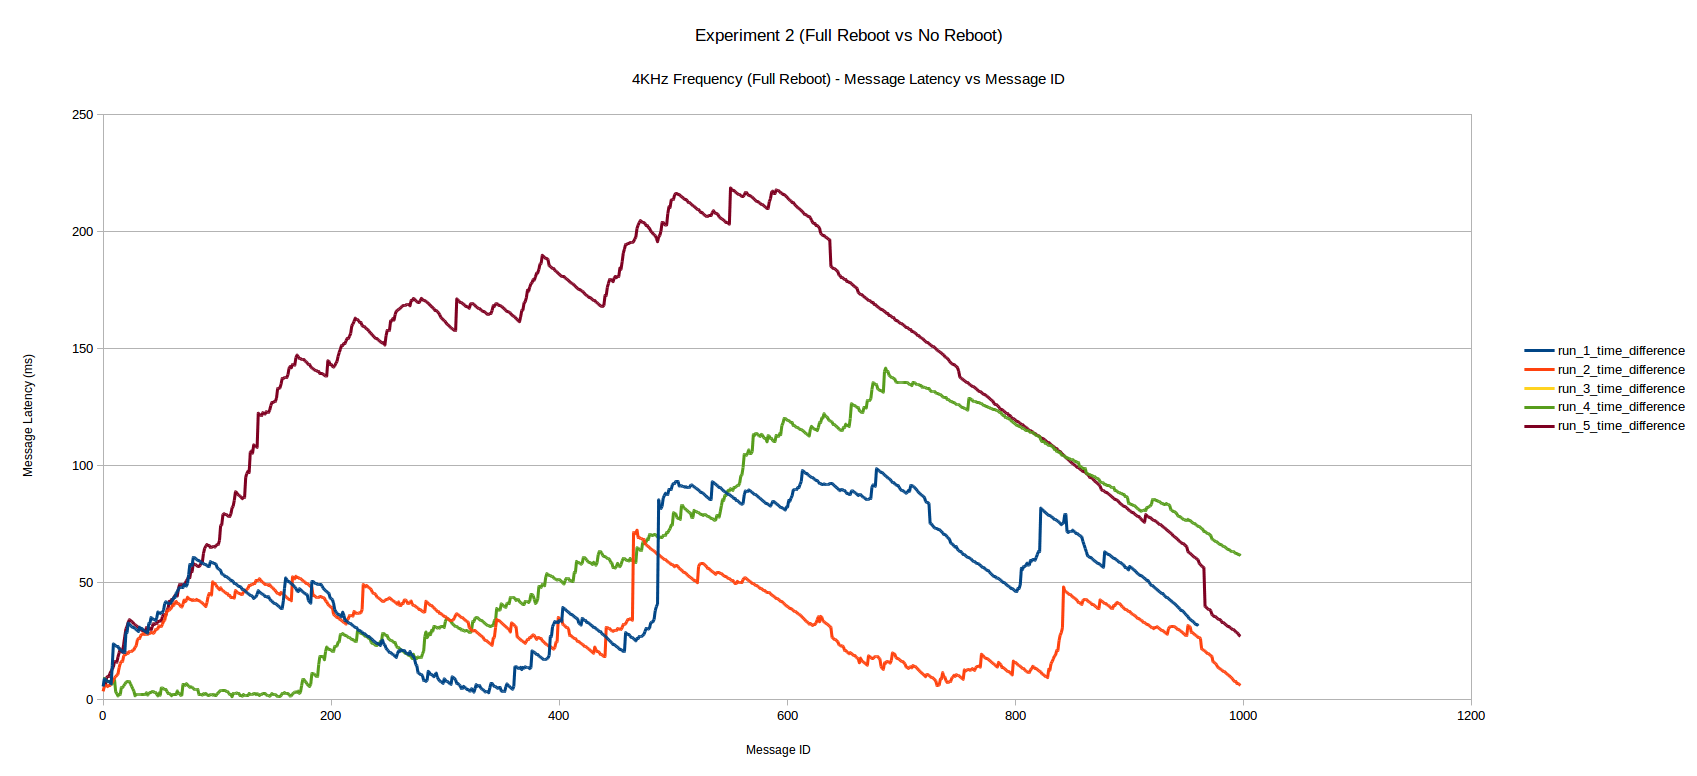
\includegraphics[width=\textwidth]{images/full-reboot-4khz.png}
\caption{Experiment 2 - Full Reboot 4KHz Message Frequency}
\label{exp2-fullreboot-4khz}
\end{figure}

\begin{figure}
\centering
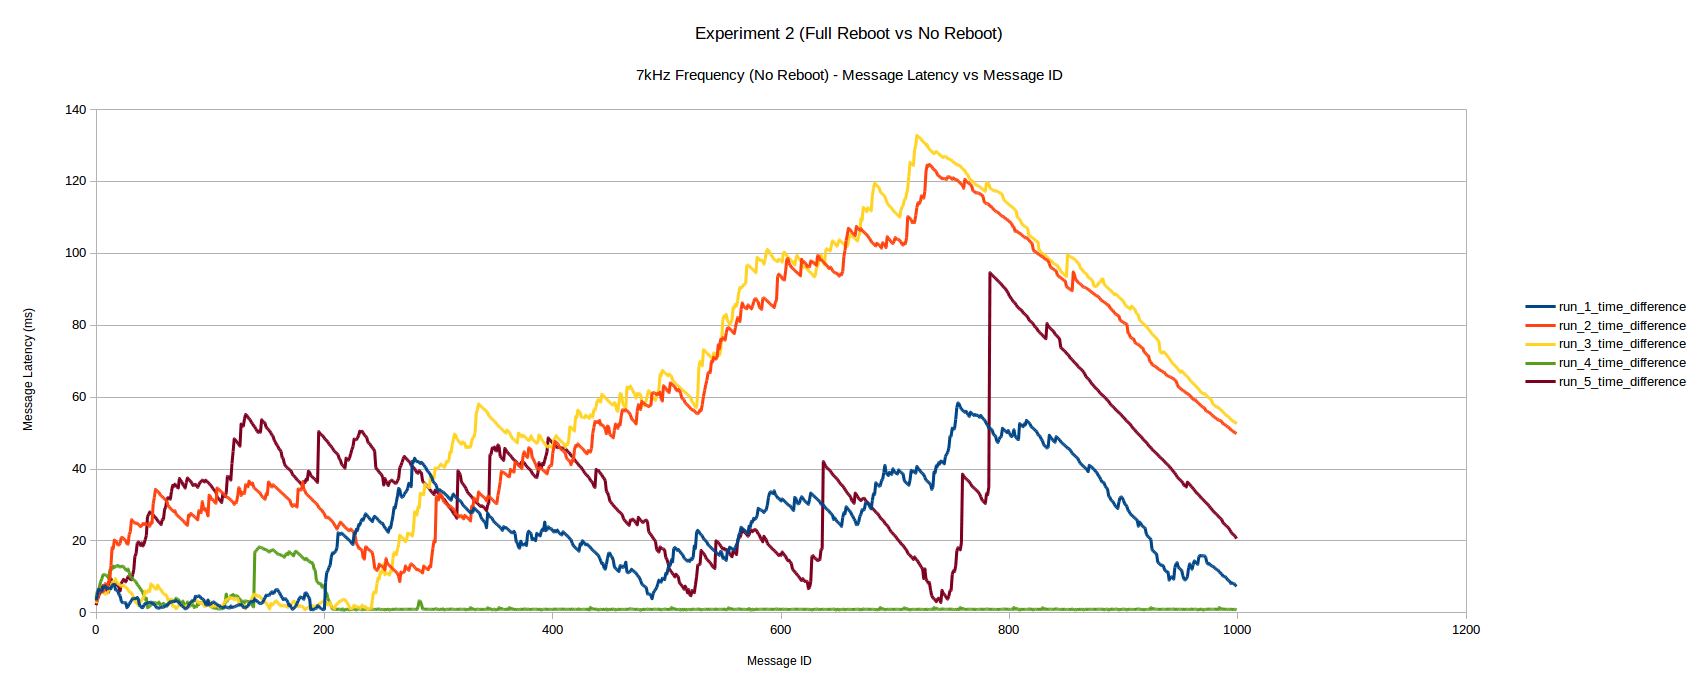
\includegraphics[width=\textwidth]{images/no-reboot-7khz.png}
\caption{Experiment 2 - No Reboot 7KHz Message Frequency}
\label{exp2-noreboot-7khz}
\end{figure}

\begin{figure}
\centering
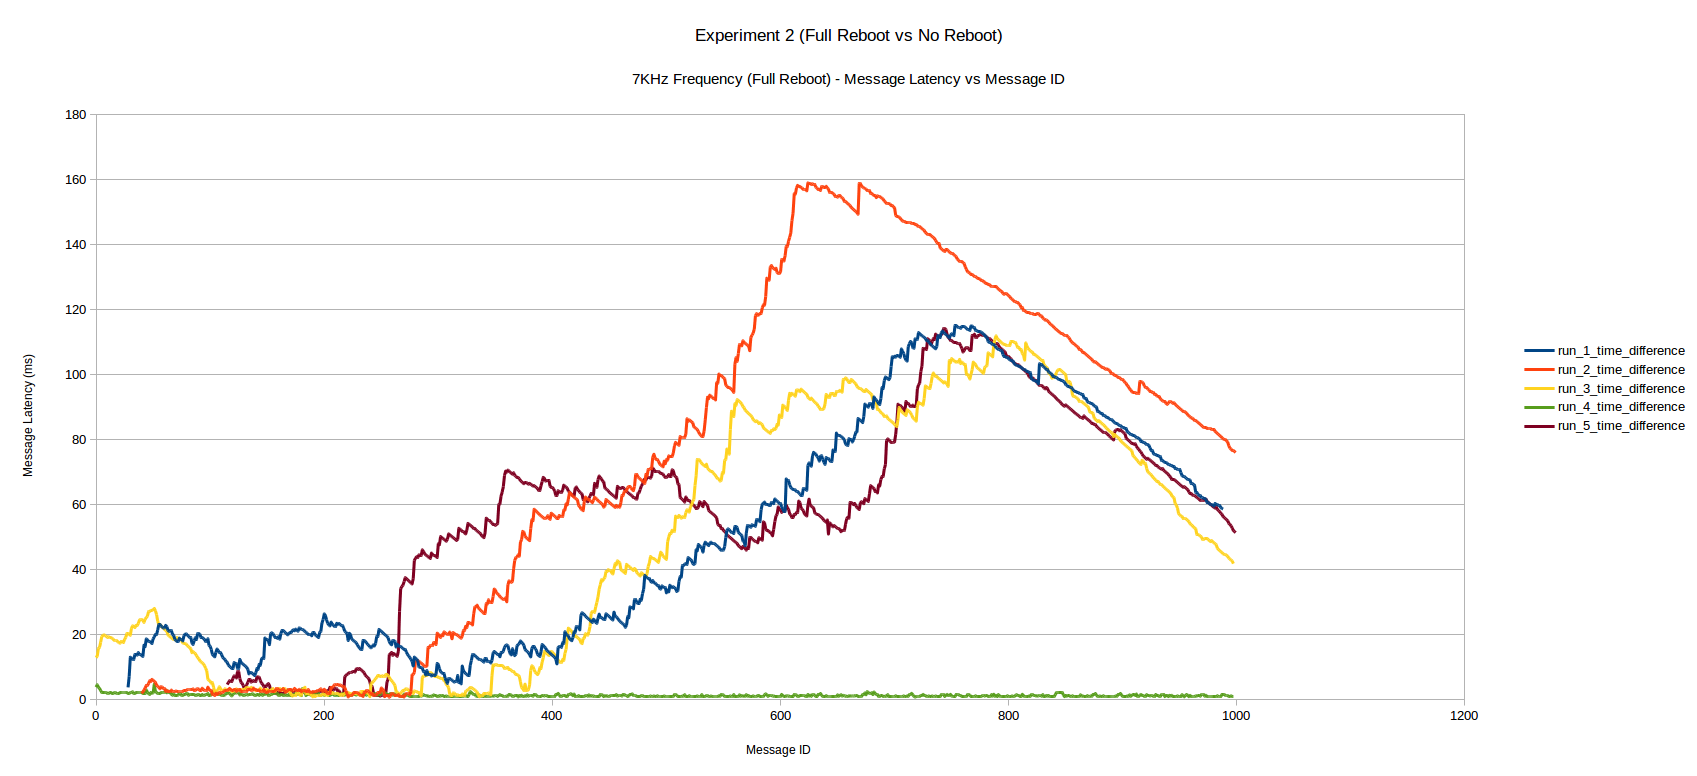
\includegraphics[width=\textwidth]{images/full-reboot-7khz.png}
\caption{Experiment 2 - Full Reboot 7KHz Message Frequency}
\label{exp2-fullreboot-7khz}
\end{figure}

\begin{figure}
\centering
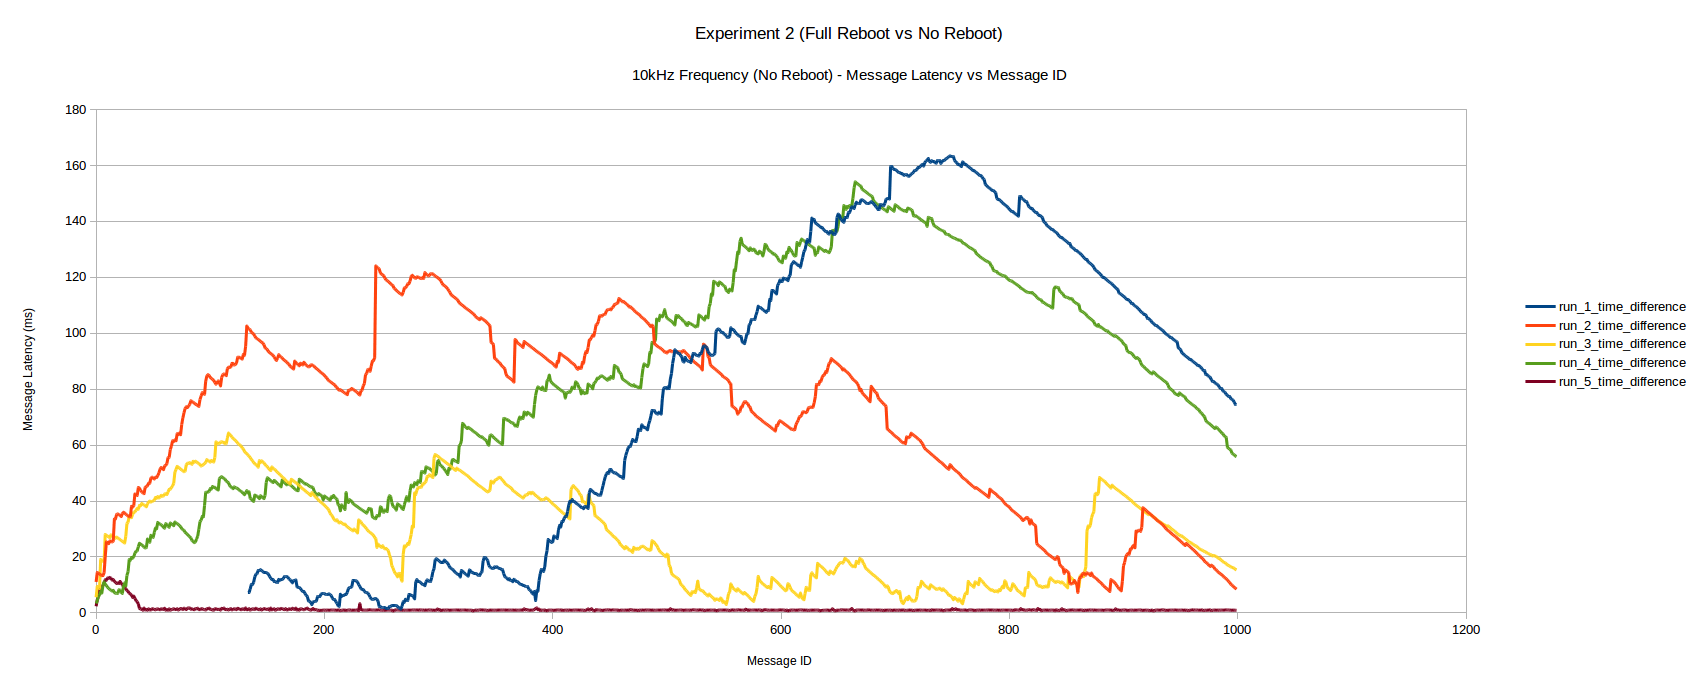
\includegraphics[width=\textwidth]{images/no-reboot-10khz.png}
\caption{Experiment 2 - No Reboot 10KHz Message Frequency}
\label{exp2-noreboot-10khz}
\end{figure}

\begin{figure}
\centering
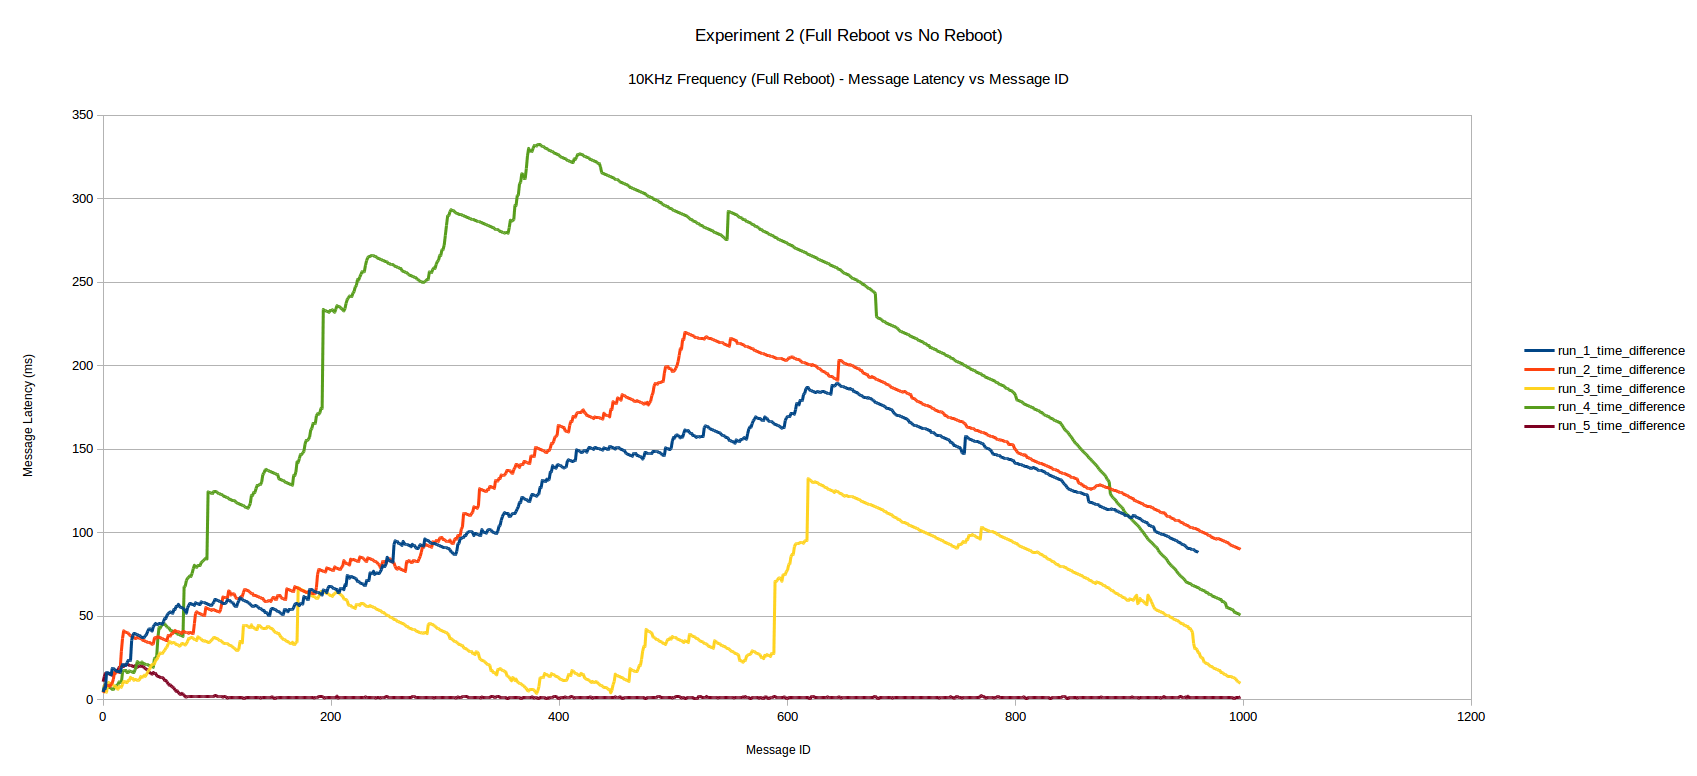
\includegraphics[width=\textwidth]{images/full-reboot-10khz.png}
\caption{Experiment 2 - Full Reboot 10KHz Message Frequency}
\label{exp2-fullreboot-10khz}
\end{figure}
\fi
\chapter{Code}

\section{Experiment 1 - Initial Code}
\label{Exp1InitCode}

\subsection{Sender and Receiver}

Code commented out.
\iffalse
\begin{lstlisting}[language=Python]
#!/usr/bin/env python

import rospy
from rosberry_experiments.msg import StampedMessage
import time
import sys

N = None
RATE = None
f = None

def listener(msg):
    recv_time = rospy.get_rostime()
    send_time = msg.t

    f.write(str(msg.id))
    f.write(",")
    f.write(str(send_time))
    f.write(",")
    f.write(str(recv_time))
    f.write("\n")

def talker():
    pub = rospy.Publisher('chatter_m', StampedMessage, queue_size=RATE)
    rospy.init_node('talker', anonymous=True)
    rate = rospy.Rate(RATE)
    for i in xrange(N):
        hello_str = "hello world"
        timestamp = rospy.get_rostime()
        pub.publish(id=i, t=timestamp ,message=hello_str )
        rate.sleep()

def main():
    global RATE, N, f
    RATE = int(sys.argv[1])
    N = int(sys.argv[2])
    f = open("times_"+str(RATE)+".txt", "w+")
    print RATE, N
    try:
        sub = rospy.Subscriber("chatter_s", StampedMessage, listener)
        talker()
        rospy.sleep(5)
        f.close()
    except rospy.ROSInterruptException:
        pass


if __name__ == '__main__':
    main()
\end{lstlisting}

\subsection{Echoer}
\begin{lstlisting}[language=Python]
#!/usr/bin/env python

import rospy
from rosberry_experiments.msg import StampedMessage
import time
import sys

RATE = None

def listener(msg, args):
    rate = rospy.Rate(RATE)
    pub = args[0]
    pub.publish(msg)
    rate.sleep()

def main():
    global RATE
    RATE = int(sys.argv[1])
    try:
        rospy.init_node('talker1', anonymous=True)
        pub = rospy.Publisher('chatter_s', StampedMessage, queue_size=RATE)
        sub = rospy.Subscriber("chatter_m", StampedMessage, listener, callback_args=[pub])
        rospy.spin()
    except rospy.ROSInterruptException:
        pass

if __name__ == '__main__':
    main()
\end{lstlisting}

\section{Experiment 1 - Revised Code}

\subsection{Sender and Receiver}
\begin{lstlisting}[language=Python]
#!/usr/bin/env python

import rospy
from rosberry_experiments.msg import StampedMessage
import time
import sys

N = None
RATE = None
f = None

def listener(msg):
    recv_time = rospy.get_rostime()
    sent_time = msg.t
    f.write(str(msg.id) + "," + str(sent_time) + "," + str(recv_time) + "\n")

def talker():
    pub = rospy.Publisher('chatter_m', StampedMessage, queue_size=N)
    rospy.init_node('talker', anonymous=True)
    rate = rospy.Rate(RATE)
    for i in xrange(N):
        hello_str = "hello world"
        timestamp = rospy.get_rostime()
        pub.publish(id=i, t=timestamp, message=hello_str )

        rate.sleep()

def main():
    global RATE, N, f
    RATE = int(sys.argv[1])
    N = int(sys.argv[2])
    f = open("times_"+str(RATE)+".txt", "w+")
    print RATE, N
    try:
        sub = rospy.Subscriber("chatter_s", StampedMessage, listener)
        talker()
        rospy.sleep(5)
        f.close()

    except rospy.ROSInterruptException:
        print "Exception: ROSInterruptException"


if __name__ == '__main__':
    main()
\end{lstlisting}

\subsection{Echoer}
\begin{lstlisting}[language=Python]
#!/usr/bin/env python

import rospy
from rosberry_experiments.msg import StampedMessage
import time
import sys

def listener(msg, args):
    pub = args[0]
    pub.publish(msg)

def main():
    N = int(sys.argv[2])
    rospy.init_node('talker1', anonymous=True)
    pub = rospy.Publisher('chatter_s',
						StampedMessage, queue_size=N)

    sub = rospy.Subscriber("chatter_m",
						StampedMessage, listener, callback_args=[pub])
    try:
        rospy.spin()
    except rospy.ROSInterruptException:
        print "Exception: ROSInterruptException"

if __name__ == '__main__':
    main()
\end{lstlisting}
\fi
\chapter{Running the Programs}

To compile this dissertation:
\begin{verbatim}

	> pdflatex dissertation
	> bibtex dissertation
	> pdflatex dissertation
    > pdflatex dissertation

\end{verbatim}


An example of running from the command line is as follows:
\begin{verbatim}
	> rosrun rosberry_experiments run_experiment.py
\end{verbatim}


\chapter{Generating Random Graphs (Example Appendix)}
\label{sec:randomGraph}

\begin{verbatim}
	> java RandomGraph 100 0.9 > 100-90-00.clq
\end{verbatim}
\end{appendices}

%%%%%%%%%%%%%%%%%%%%
%   BIBLIOGRAPHY   %
%%%%%%%%%%%%%%%%%%%%

\bibliographystyle{plain}
\bibliography{bib}

\end{document}
